%   File: BasisIndependentDotCross.tex
% Author: Adam Leeper (with modifications by Paul Mitiguy)
%------------------------------------------------------------------------------
%\\[0.45pc]
\providecommand{\isolatedBuild}[1]{#1}% Fallback definition to build normally.
\isolatedBuild{
  \documentclass[11pt,letterpaper]{book}
  %\documentclass[11pt,letterpaper]{book}

% aleeper: I think these are needed for Paul's macros?
\usepackage{epsfig}
\usepackage{epstopdf}

%\makeatletter
%\typeout{The import path is \import@path}
%\makeatother

\usepackage{import}

\subimport{./}{packagesMitiguy.sty}
\subimport{./}{macrosMitiguy.tex}
\subimport{./}{PageStylesMitiguy.tex}
\subimport{./}{macrosLeeper.tex}
   % Found via TEXINPUTS environment variable.
  \isolatedBuildHeader{Vector Basics Examples}
                      {Vector Basics - Distributive Rule for Dot and Cross}
}
%%%
%%%
%%%
\begin{minipage}[t]{0.55\linewidth}
  \minipageTopAnchor
  %
  %\vspace*{-0.2cm}
  The figure to the right shows \boldUnderlineDarkRed{unit} vectors
  \/ \uvecHat{v}, \uvecHat{w}, \uvecHat{x}, \uvecHat{y}, \uvecHat{z}.
  \\[0.00pc] The angle between adjacent vectors is $\degrees{30}$.
  %
  \begin{displaymath}
    \textrm{Given:}
    \hspace{0.65cm}
    \bvec{a} \equals[\;] 0.5\,\uvecHat{y} \plus[\;]  2\,\uvecHat{w}
    \hspace{1.65cm}
    \bvec{b} \equals[\;]   2\,\uvecHat{v} \minus[\;] 1\,\uvecHat{x}
    \hspace*{0.85cm}
  \end{displaymath}
  %
\end{minipage}
\hfill
\begin{minipage}[t]{0.44\linewidth}
  \minipageTopAnchor
  %\vspace*{-1cm}
  \begin{center}
    \includegraphicsAB[width=0.66\linewidth]
      {basis_independent_vectors_sketch.png}
      {basis_independent_vectors.png}
  \end{center}
\end{minipage}

\begin{enumerate}
  \setlength{\itemsep}{0.35pc}
    %
  \item \boldUnderlineDarkRed{Draw} vectors \bvec{a} and \bvec{b} on the figure.
    %
  \item Dot product can be regarded as a
    ``\newnameIndex{projection}{measure of a vector (positive/negative)}''
    \/ or
    ``\newnameIndex{measure}{measure of a vector (positive/negative)}''
    \/ of a vector in the direction of a unit vector.
    \\[0.0pc]
    \/ \boldUnderlineDarkRed{Draw} \/ $\bvec{a} \DotProduct[\:\:] \uvecHat{x}$,
    \/ the projection of \bvec{a} on \uvecWithHat{x}
    \/ \smallerDescriptionParens[\small]{the \uvecWithHat{x} measure of
    \bvec{a}}.
    %
  \item Use the vector dot-product \boldDarkRed{distributive property} to
    calculate \/ $\bvec{a} \DotProduct[\;] \uvecHat{x}$.
    %
    \\[0.0pc]\textbf{Result:}\\[-0.65pc]
    %
    \begin{displaymath}
      \bvec{a} \DotProduct[\;] \uvecHat{x} \equals[\;]
      \hidemath[2cm]{2.5 \mult[\;] \cos(\degrees{30}) \equals[\;] 2.17}
    \end{displaymath}
      %
      \Solution{}{0.99\linewidth}{
        \begin{minipage}{0.65\linewidth}
        \begin{tabular}{@{}l@{ \equals[\;] }ll}
          $\bvec{a} \cdot \uvecHat{x}$
          & $(0.5~\uvecHat{y} \plus[\;] 2~\uvecHat{w}) \cdot \uvecHat{x}$
          &
          \\[1.0pc]
          & $0.5~\uvecHat{y} \cdot \uvecHat{x}
            \plus[\;] 2~\uvecHat{w} \cdot \uvecHat{x}$
          & distribute
          \\[1.0pc]
          &
          $0.5 * \magnitude{\uvecHat{y}} \magnitude{\uvecHat{x}}
            \cos\angle(\uvecHat{y},\uvecHat{x})
            \plus[\;] 2 ~\magnitude{\uvecHat{w}}
            \magnitude{\uvecHat{x}} \cos\angle(\uvecHat{w},\uvecHat{x})$
          & definition
          \\[1.0pc]
          & $0.5*(1)(1)\cos\degrees{30}
          \plus[\;] 2*(1)(1)\cos\degrees{30}$
          & plug in
          \\[1.0pc]
          & $2.5*\cos(\degrees{30})$
          & simplify
          \\[1.0pc]
          & $2.17$
          &
        \end{tabular}
        \end{minipage}
        \begin{minipage}{0.34\linewidth}
          \minipageTopAnchor
          \flushright
          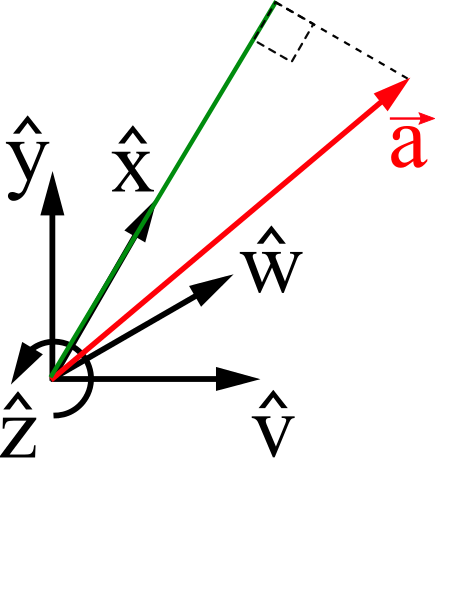
\includegraphics[width=0.6\linewidth]
            {basis_independent_vectors_projection.png}
          \\[0.0pc]
          2.17 is the \boldDarkGreen{\underline{length}} of the green line.
        \end{minipage}
        \\[0.45pc]
      }
      %
%-----------------
%\begin{comment}
%-----------------
  \item Use the vector cross-product \boldDarkRed{distributive property} to
    calculate \/ $\bvec{a} \CrossProduct[\;] \bvec{b}$.
    %
    \\[0.0pc]\textbf{Result:}\\[-0.65pc]
    %
    \begin{displaymath}
      \bvec{a} \CrossProduct[\;] \bvec{b} \equals[\;]
      \hidemath[2cm]{-3.75~\uvecHat{z}}
    \end{displaymath}
    %
    \Solution{}{0.99\linewidth}{
      %\\[0.0pc]
      \begin{tabular}{@{}l@{ \equals[\;] }ll}
        $\bvec{a} \times \bvec{b}$ &
        $(0.5~\uvecHat{y} \plus[\;] 2~\uvecHat{w}) \times (2~\uvecHat{v} - 1~\uvecHat{x})$
        &
        \\[1.0pc]
        & $1~\uvecHat{y} \times \uvecHat{v} \minus[\;] 0.5~\uvecHat{y} \times \uvecHat{x}
        \plus[\;] 4~\uvecHat{w} \times \uvecHat{v} - 2~\uvecHat{w} \times \uvecHat{x}$
        & distribute
        \\[1.0pc]
        & $1~(-\uvecHat{z}) \minus[\;] 0.5~(-\uvecHat{z}) \sin\angle(\uvecHat{y}, \uvecHat{x})
        \plus[\;] 4~(-\uvecHat{z})\sin\angle(\uvecHat{w}, \uvecHat{v}) - 2~(+\uvecHat{z})\sin\angle(\uvecHat{w}, \uvecHat{x})$
        & definition
        \\[1.0pc]
        & $-1~\uvecHat{z} \plus[\;] 0.5\sin\degrees{30}~\uvecHat{z}
        \minus[\;] 4~\sin\degrees{30}~\uvecHat{z} - 2~\sin\degrees{30}~\uvecHat{z}$
        & plug in
        \\[1.0pc]
        & $-3.75~\uvecHat{z}$
        \hspace{0.5cm}
        (Note the result of a cross product must be a
        \boldDarkRed{\underline{vector}}.)
        & simplify
      \end{tabular}
    }
    %
%-----------------
%\end{comment}
%-----------------
\end{enumerate}
%
\isolatedBuildFooter